\subsubsection{CreateListView}

\label{CreateListView}
\begin{figure}[ht]
	\centering
	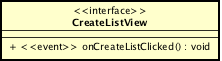
\includegraphics[scale=0.5]{Sezioni/SottosezioniST/img/app/CreateListView.png}
	\caption{CreateListView}
\end{figure}

\begin{itemize}
\item \textbf{Descrizione}: Interfaccia che estende \texttt{GeneralView} che una volta implementata permette al presenter e allo sviluppatore di personalizzare la vista dedicata alla creazione di una nuova lista.
\item \textbf{Utilizzo}: L'interfaccia viene utilizzata per disaccoppiare presenter e implementazione della vista, e visualizza i dati che gli vengono passati dal presenter.
\item \textbf{Attributi}:
\item \textbf{Metodi}:
\item \textbf{Eventi}:
	\begin{itemize}
	\item \textit{public onCreateListClicked():void}\\
	Evento che rappresenta il click sul bottone dedicato alla creazione di una nuova lista, dopo il quale si può procedere con la creazione della nuova lista.
	\end{itemize}
\end{itemize}

\subsubsection{CreateListViewImpl}

\label{CreateListViewImpl}
\begin{figure}[ht]
	\centering
	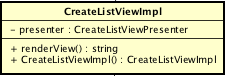
\includegraphics[scale=0.5]{Sezioni/SottosezioniST/img/app/CreateListViewImpl.png}
	\caption{CreateListViewImpl}
\end{figure}

\begin{itemize}
\item \textbf{Descrizione}: Classe che implementa l'interfaccia \texttt{CreateListView}, che permette al presenter e allo sviluppatore di personalizzare la vista dedicata alla creazione di una nuova lista.
\item \textbf{Utilizzo}: Classe utilizzata per creare una nuova lista permettendo di personalizzarne la view.
\item \textbf{Attributi}: 
	\begin{itemize}
	\item \textit{private presenter:CreateListViewPresenter}\\
	Il presenter associato alla view per creare una nuova lista, al quale questa classe delega la gestione del comportamento della view stessa.
	\end{itemize}
\item \textbf{Metodi}:
	\begin{itemize}
	\item \textit{public CreateListViewImpl():CreateListViewImpl}\\
	Il costruttore della classe CreateListViewImpl.
	\item \textit{public renderView():string}\\
		Genera il codice HTML CSS JS necessario per visualizzare la view.
	\end{itemize}
\item \textbf{Eventi}:
\end{itemize}

\subsubsection{CreateListViewPresenter}

\label{CreateListViewPresenter}
\begin{figure}[ht]
	\centering
	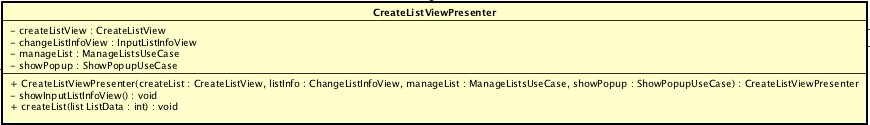
\includegraphics[scale=0.5]{Sezioni/SottosezioniST/img/app/CreateListViewPresenter.png}
	\caption{CreateListViewPresenter}
\end{figure}

\begin{itemize}
\item \textbf{Descrizione}: Classe che rappresenta il presenter dedicato alla view per la creazione di una nuova lista.
\item \textbf{Utilizzo}: Il presenter fa da tramite tra l'implementazione della view e la parte logica dell'applicazione, formattando i dati che verranno visualizzati nella view e manipolando gli input dell'utente per eseguire le operazioni predisposte.
\item \textbf{Attributi}: 
	\begin{itemize}
	\item \textit{private createListView:CreateListView}\\
	La view associata al presenter.
	\item \textit{private changeListInfoView:InputListInfoView}\\
	Vista che permette l'input dei dati relativi ad una lista.
	\item \textit{private manageList:ManageListUseCase}\\
	Oggetto dedicato alla gestione dei dati relativi alla lista all'interno del database.
	\item \textit{private showPopup:ShowPopupUseCase}\\
	Oggetto dedicato alla creazione del popup per la creazione della lista.
	\end{itemize}
\item \textbf{Metodi}:
	\begin{itemize}
	\item \textit{public CreateListViewPresenter(createList:CreateListView, listInfo:ChangeListInfoView, manageList:ManageListsUseCase, showPopup:ShowPopupUseCase):CreateListViewPresenter}\\
		Il Costruttore del presenter CreateListViewPresenter.
		\item{\textbf{Parametri}: \begin{itemize}
		\item \textit{createList:CreateListView}\\
			La view associata al presenter.
		\item \textit{listInfo:ChangeListInfoView}\\
			Vista che permette l'input dei dati relativi ad una lista.
		\item \textit{manageList:ManageListsUseCase}\\
			Oggetto dedicato alla gestione dei dati relativi alla lista all'interno del database.
		\item \textit{showPopup:ShowPopupUseCase}\\
			Oggetto che permette creazione di un popup per l'immissione dei dati della lista da creare.
		\end{itemize}}
	\item \textit{private showInputListInfoView():void}\\
	 Metodo che permette di mostrare la vista attraverso la quale l'utente potrà andare a modificare i dati della lista.
	\item \textit{public createList(list:ListData):void}\\
	Metodo che crea la nuova lista.
			\item{\textbf{Parametri}: \begin{itemize}
			\item \textit{list:ListData}\\
			Insieme di tutti i dati e le informazioni di una lista.
			\end{itemize}}
	\end{itemize}
\item \textbf{Eventi}:
\end{itemize}

\subsubsection{InputListInfoView}

\label{InputListInfoView}
\begin{figure}[ht]
	\centering
	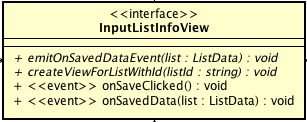
\includegraphics[scale=0.5]{Sezioni/SottosezioniST/img/app/InputListInfoView.png}
	\caption{InputListInfoView}
\end{figure}

\begin{itemize}
\item \textbf{Descrizione}: Questa interfaccia rappresenta la view relativa al popup per l'immissione, rimozione o modifica di tutti i dati relativi alla lista.
\item \textbf{Utilizzo}: L'interfaccia viene utilizzata per disaccoppiare presenter e implementazione della vista, e visualizza i dati che gli vengono passati dal presenter.
\item \textbf{Attributi}: 
\item \textbf{Metodi}:
	\begin{itemize}	
	\item \textit{public emitOnSavedDataEvent(list:ListaData):void}\\
	Metodo necessario al presenter per far emettere alla view l'evento onSavedData(list:ListData), notificando tutti gli oggetti in ascolto che la lista è stata salvata con successo.
			\item{\textbf{Parametri}: \begin{itemize}
			\item \textit{list:ListaData}\\
			Insieme di tutti i dati e le informazioni di una lista.
			\end{itemize}}
	\item \textit{public createViewForListWithId(listId:string):void}\\
	Metodo che permette di creare una una view per visualizzarli.
			\item{\textbf{Parametri}: \begin{itemize}
			\item \textit{listId:string}\\
			Parametro che rappresenta l'id della lista di cui si vuole creare in una view.
			\end{itemize}}
	\end{itemize}
\item \textbf{Eventi}:
	\begin{itemize}
	\item \textit{public onSaveClicked():void}\\
	Evento emesso dalla view che rappresenta interazione di un utente con un bottone dedicato al salvataggio della lista.
	\item \textit{public onSavedData(list:ListData):void}\\
			Evento che notifica tutti gli oggetti in ascolto che la lista è stata salvata con successo.
			\item{\textbf{Parametri}: \begin{itemize}
			\item \textit{list:ListData}\\
			Insieme di tutti i dati e le informazioni di una lista.
			\end{itemize}}
	\end{itemize}
\end{itemize}

\subsubsection{ManageListsUseCase}

\label{ManageListsUseCase}
\begin{figure}[ht]
	\centering
	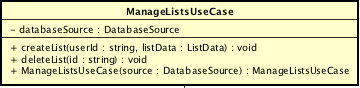
\includegraphics[scale=0.5]{Sezioni/SottosezioniST/img/app/ManageListsUseCase.png}
	\caption{ManageListsUseCase}
\end{figure}

\begin{itemize}
\item \textbf{Descrizione}: Classe che permette di gestire i dati relativi alle liste all'interno del database.
\item \textbf{Utilizzo}: Classe utilizzata per eliminare o aggiungere una lista al database.
\item \textbf{Attributi}: 
	\begin{itemize}
	\item \textit{private databaseSource:DatabaseSource}\\
		Riferimento al database.
	\end{itemize}
\item \textbf{Metodi}:
	\begin{itemize}
	\item \textit{public createList(userId:string,listData:ListData):void}\\
		Metodo dedicato alla creazione della lista nel database.
			\item{\textbf{Parametri}: \begin{itemize}
			\item \textit{userId:string}\\
			Id dell'utente.
			\item \textit{listData:ListData}
			Insieme di tutti i dati e le informazioni della lista.
			\end{itemize}}
	\item \textit{public deleteList(id:string):void}\\
	Metodo dedicato alla rimozione dal database della lista.
			\item{\textbf{Parametri}: \begin{itemize}
			\item \textit{id:string}\\
			Id della lista da rimuovere.
			\end{itemize}}
	\item \textit{public ManageListsUseCase(source:DatabaseSource):ManageListsUseCase}\\
	Il costruttore della classe ManageListsUseCase.
		\item{\textbf{Parametri}: \begin{itemize}
			\item \textit{source:DatabaseSource}\\
						Riferimento al database.
			\end{itemize}}
	\end{itemize}
\item \textbf{Eventi}:
\end{itemize}

\subsubsection{DeleteListView}

\label{DeleteListView}
\begin{figure}[ht]
	\centering
	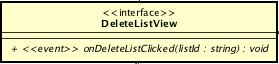
\includegraphics[scale=0.5]{Sezioni/SottosezioniST/img/app/DeleteListView.png}
	\caption{DeleteListView}
\end{figure}

\begin{itemize}
\item \textbf{Descrizione}: Interfaccia che estende \texttt{GeneralView} che una volta implementata permette al Presenter e allo sviluppatore di personalizzare la vista dedicata all'eliminazione di una lista.
\item \textbf{Utilizzo}: L'interfaccia viene utilizzata per disaccoppiare presenter e implementazione della vista, e visualizza i dati che gli vengono passati dal presenter.
\item \textbf{Attributi}: 
\item \textbf{Metodi}:
\item \textbf{Eventi}:
	\begin{itemize}
	\item \textit{public onDeleteListClicked(listId:string):void}\\
	Evento che rappresenta il click sul bottone dedicato all'eliminazione di una lista, dopo il quale verrà eliminata la lista.
	\item{\textbf{Parametri:} \begin{itemize}
	\item \textit{listId:string}
	Parametro che rappresenta l'id della lista che si vuole eliminare.
	\end{itemize}}
	\end{itemize}
\end{itemize}

\subsubsection{DeleteListViewImpl}

\label{DeleteListViewImpl}
\begin{figure}[ht]
	\centering
	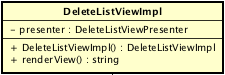
\includegraphics[scale=0.5]{Sezioni/SottosezioniST/img/app/DeleteListViewImpl.png}
	\caption{DeleteListViewImpl}
\end{figure}

\begin{itemize}
\item \textbf{Descrizione}: Classe che implementa l'interfaccia \texttt{DeleteListView}, che permette al Presenter e allo sviluppatore di personalizzare la vista dedicata all'eliminazione di una lista.
\item \textbf{Utilizzo}:
\item \textbf{Attributi}: 
	\begin{itemize}
	\item \textit{private presenter:DeleteListViewPresenter}\\
		Il presenter relativo alla view per l'eliminazione di una lista.
	\end{itemize}
\item \textbf{Metodi}:
	\begin{itemize}
	\item \textit{public DeleteListViewImpl():DeleteListViewImpl}\\
	Il costruttore della classe DeleteListViewImpl.
	\item \textit{public renderView():string}\\
			Genera il codice HTML CSS JS necessario per visualizzare la view.
	\end{itemize}
\item \textbf{Eventi}:
\end{itemize}

\subsubsection{DeleteListViewPresenter}

\label{DeleteListViewPresenter}
\begin{figure}[ht]
	\centering
	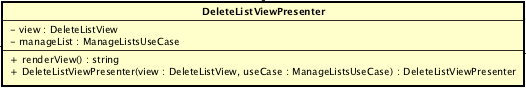
\includegraphics[scale=0.5]{Sezioni/SottosezioniST/img/app/DeleteListViewPresenter.png}
	\caption{DeleteListViewPresenter}
\end{figure}

\begin{itemize}
\item \textbf{Descrizione}: 
\item \textbf{Utilizzo}: Il presenter fa da tramite tra l'implementazione della view e la parte logica, formattando i dati che verranno visualizzati nella view e manipolando gli input dell'utente per eseguire le operazioni predisposte.
\item \textbf{Attributi}: 
	\begin{itemize}
	\item \textit{private view:DeleteListView}\\
		La view associata al presenter.
	\item \textit{private manageList:ManageListUseCase}\\
				Oggetto dedicato alla gestione dei dati relativi alla lista all'interno del database.
	\end{itemize}
\item \textbf{Metodi}:
	\begin{itemize}
	\item \textit{public renderView():string}\\
	Genera il codice HTML CSS JS necessario per visualizzare la view.
	\item \textit{public DeleteListViewPresenter(view:DeleteListView, useCase:ManageListsUseCase):DeleteListViewPresenter}\\
	Il Costruttore del presenter DeleteListViewPresenter.
		\item{\textbf{Parametri}: \begin{itemize}
		\item \textit{view:DeleteListView}\\
			La view associata al presenter.
		\item \textit{useCase:ManageListsUseCase}\\
			Oggetto dedicato alla gestione dei dati relativi alla lista all'interno del database.
		\end{itemize}}
	\end{itemize}
\item \textbf{Eventi}:
\end{itemize}